\documentclass[11pt,a4paper]{article}

% ---------------------------
% Packages
% ---------------------------
\usepackage[a4paper,margin=1in]{geometry}
\usepackage[T1]{fontenc}
\usepackage{lmodern}
\usepackage{microtype}
\usepackage{graphicx}
\usepackage{caption}
\usepackage{subcaption}
\usepackage{booktabs}
\usepackage{array}
\usepackage{amsmath}
\usepackage{enumitem}
\usepackage{hyperref}
\usepackage{xcolor}
\usepackage{fancyhdr}
\usepackage{titlesec}

% ---------------------------
% Hyperref setup
% ---------------------------
\hypersetup{
	colorlinks=true,
	linkcolor=blue,
	urlcolor=blue,
	citecolor=blue
}

% ---------------------------
% Header / Footer
% ---------------------------
\pagestyle{fancy}
\fancyhf{}
\lhead{\textbf{Static PAT vs Dynamic PAT in Backend Manufacturing}}
\rhead{\textbf{White Paper}}
\cfoot{\thepage}

% ---------------------------
% Section formatting
% ---------------------------
\titleformat{\section}{\large\bfseries}{\thesection.}{0.5em}{}
\titleformat{\subsection}{\normalsize\bfseries}{\thesubsection.}{0.5em}{}

% ---------------------------
% Title
% ---------------------------
\title{\textbf{Static Part Average Testing (SPAT) \\ vs \\Dynamic Part Average Testing (DPAT)}\\
	\large Why Dynamic PAT Can Become Less Reliable in Semiconductor Backend Assembly \& Test}
\author{Viren Patel\\
	\small \textit{Decoded with Viren — Technical White Paper}}
\date{\today}

\begin{document}
	\maketitle
	
	\vspace{-0.5em}
	
	% ---------------------------
	% Disclaimer (important for IP safety)
	% ---------------------------
	\begin{center}
		\fbox{
			\begin{minipage}{0.95\linewidth}
				\small
				\textbf{Disclaimer:} This document is based on public engineering principles and author-developed models.
				All scenarios, datasets, and results are illustrative and/or simulated and do not represent any specific
				company, customer, product, test limits, or proprietary manufacturing process. Views are the author’s own.
			\end{minipage}
		}
	\end{center}
	
	\vspace{1em}
	
	% ---------------------------
	% Abstract
	% ---------------------------
	\begin{abstract}
		Part Average Testing (PAT) is widely used in semiconductor backend test to screen abnormal parts using
		parametric outlier detection. Two commonly deployed methodologies are \textbf{Static Part Average Testing (SPAT)},
		where limits are derived from large historical production datasets, and \textbf{Dynamic Part Average Testing (DPAT)},
		where limits are updated adaptively using recent test windows (e.g., rolling lots or time windows).
		While DPAT can offer faster reaction time to localized shifts, this paper argues that DPAT can become
		\textbf{less reliable and less effective in backend assembly and test environments} due to stacked variability sources
		(materials, firmware configurations, equipment/toolchain drift, measurement noise, and routing/rework variation).
		Conversely, SPAT provides improved screening stability and scalability in high-mix backend conditions by
		anchoring acceptance limits to large-volume population behavior. DPAT becomes most effective only when backend
		conditions are \textbf{ultra-stable and fully traceable}.
	\end{abstract}
	
	\tableofcontents
	\newpage
	
	% ---------------------------
	\section{Introduction}
	Semiconductor backend manufacturing (Assembly \& Test) is a high-variance environment compared to wafer fab.
	Product performance and measured parametric results are influenced not only by silicon behavior, but also by:
	materials and packaging variations, firmware and calibration routines, equipment differences, thermal handling,
	test program changes, contactor/socket wear, measurement system repeatability (GR\&R), and routing/rework history.
	
	Because PAT is intended to screen abnormal parts and provide early detection of distribution-level changes,
	the choice between SPAT and DPAT significantly impacts yield stability, false reject risk, and debug cycle time.
	
	\subsection{Key thesis}
	\textbf{DPAT only works reliably when the system is stable and traceable.}
	Backend environments are inherently multi-variable; therefore DPAT can become noisy and misleading.
	In such conditions, SPAT is generally more robust as a primary screening gate.
	
	% ---------------------------
	\section{Definitions and Terminology}
	
	\subsection{Part Average Testing (PAT)}
	PAT is an outlier-screening method applied to parametric test results to identify units that deviate
	abnormally from the population.
	
	\subsection{Static Part Average Testing (SPAT)}
	SPAT uses large historical populations (high $N$) to define stable baseline distributions and acceptance limits.
	Typical implementations use:
	\begin{itemize}[leftmargin=1.2em]
		\item Mean and standard deviation ($\mu, \sigma$) with robust variants
		\item Median and MAD-based sigma
		\item Percentile-based limits (P1/P99, etc.)
		\item Long-window control charts (EWMA/CUSUM optional)
	\end{itemize}
	
	\textbf{Interpretation:} SPAT acts as a \textbf{global population baseline}.
	
	\subsection{Dynamic Part Average Testing (DPAT)}
	DPAT calculates PAT limits using recent production results (rolling window) and can be contextualized by:
	tester ID, site, temperature, configuration, firmware revision, or routing. Typical implementations use:
	\begin{itemize}[leftmargin=1.2em]
		\item Last $N$ units or last $M$ lots
		\item Rolling time windows (e.g., last 24 hours / 7 days)
		\item Per-tool / per-site baselines
		\item Adaptive baseline updates
	\end{itemize}
	
	\textbf{Interpretation:} DPAT acts as a \textbf{local rolling baseline}.
	
	% ---------------------------
	\section{Variance Stack in Backend Assembly \& Test}
	
	Backend behavior is a stacked-variance system. Even if the silicon is stable, the measured parametric
	distribution can shift due to multiple interacting factors.
	
	\begin{figure}[h!]
		\centering
		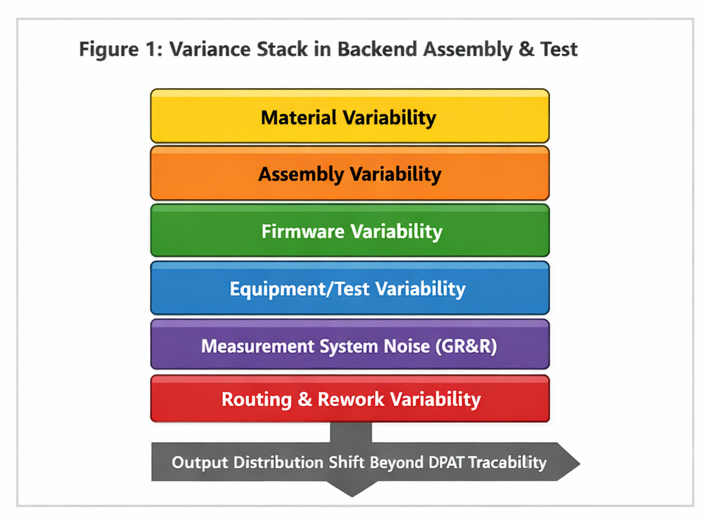
\includegraphics[width=0.92\linewidth]{figures/figure1_variance_stack.png}
		\caption{Variance stack in backend assembly \& test (illustrative).}
		\label{fig:variance_stack}
	\end{figure}
	
	\subsection{Primary variability contributors}
	\begin{enumerate}[leftmargin=1.2em]
		\item \textbf{Material variability:} suppliers, substrate lots, mold compound, solder paste, adhesives.
		\item \textbf{Assembly variability:} bonding, curing, warpage, voiding, contamination micro-variation.
		\item \textbf{Firmware variability:} FW revisions, training/calibration algorithms, trim methods.
		\item \textbf{Equipment/test variability:} tester type, socket aging, handler thermal drift, loadboard differences.
		\item \textbf{Measurement system noise:} GR\&R limitations in parametric measurement repeatability.
		\item \textbf{Routing/rework variability:} insertion history, thermal exposure differences, rework loops.
	\end{enumerate}
	
	% ---------------------------
	\section{Why DPAT Becomes Less Reliable in Backend}
	
	DPAT’s rolling baseline assumes that the most recent population represents a valid equivalence class.
	However, backend systems often violate equivalence assumptions due to incomplete traceability
	and non-linear interactions between factors.
	
	\begin{figure}[h!]
		\centering
		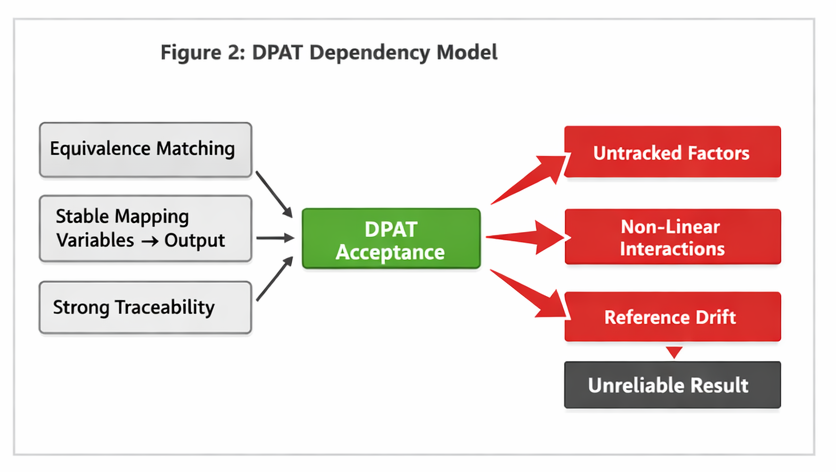
\includegraphics[width=0.92\linewidth]{figures/figure2_dpat_dependency_model.png}
		\caption{DPAT dependency model: failure modes caused by untracked factors and baseline drift.}
		\label{fig:dpat_dependency}
	\end{figure}
	
	\subsection{DPAT failure mechanisms}
	\begin{itemize}[leftmargin=1.2em]
		\item \textbf{Untracked drivers:} Many dominant backend drivers are not fully represented in traceability data.
		\item \textbf{Non-linear interactions:} e.g., FW $\times$ socket aging $\times$ temperature compensation.
		\item \textbf{Reference drift:} rolling baselines drift with equipment wear and calibration cycles.
	\end{itemize}
	
	\subsection{Risk: false rejects and false accepts}
	In high variance environments DPAT can increase both:
	\begin{itemize}[leftmargin=1.2em]
		\item \textbf{False rejects:} healthy parts rejected because baseline shifted due to noise.
		\item \textbf{False accepts:} weak parts accepted because local baseline degraded.
	\end{itemize}
	
	% ---------------------------
	\section{Why SPAT is More Robust in Backend}
	
	SPAT is anchored to large population behavior and is therefore less sensitive to short-term noise,
	temporary tester shifts, or contactor/socket wear trends. SPAT enables stable screening even across:
	\begin{itemize}[leftmargin=1.2em]
		\item multi-supplier BOM mixes,
		\item frequent routing changes,
		\item equipment heterogeneity,
		\item firmware updates across product life cycle.
	\end{itemize}
	
	% ---------------------------
	\section{SPAT vs DPAT Comparison}
	
	\begin{figure}[h!]
		\centering
		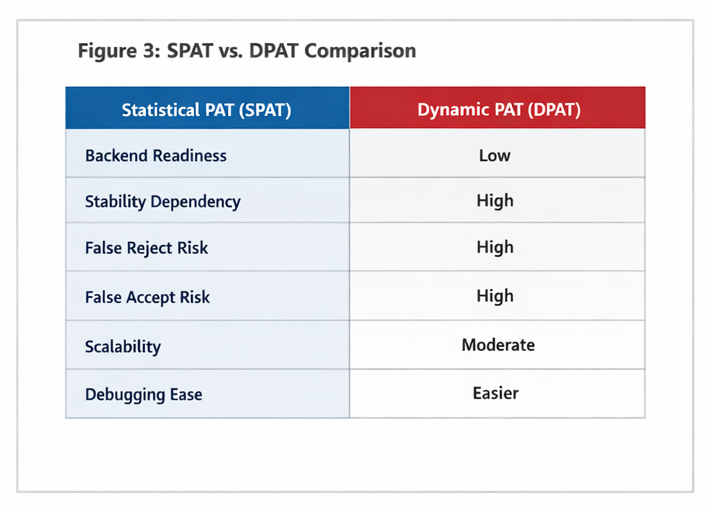
\includegraphics[width=0.92\linewidth]{figures/figure3_spat_vs_dpat_table.png}
		\caption{High-level comparison: SPAT vs DPAT for backend readiness and reliability.}
		\label{fig:comparison}
	\end{figure}
	
	% ---------------------------
	\section{When DPAT Works Best}
	
	DPAT becomes highly effective when backend conditions approximate wafer fab stability:
	\begin{itemize}[leftmargin=1.2em]
		\item minimal BOM and material variance,
		\item frozen firmware/training/calibration methods,
		\item equipment homogeneity with strong matching practices,
		\item high traceability maturity including tool capability state,
		\item controlled routing and minimized rework loops.
	\end{itemize}
	
	% ---------------------------
	\section{Recommended Hybrid PAT Framework}
	
	A practical deployment in backend uses both:
	\begin{itemize}[leftmargin=1.2em]
		\item \textbf{SPAT as primary acceptance gate} (robust global screening),
		\item \textbf{DPAT as targeted diagnostic layer} (fast local anomaly detection).
	\end{itemize}
	
	\begin{figure}[h!]
		\centering
		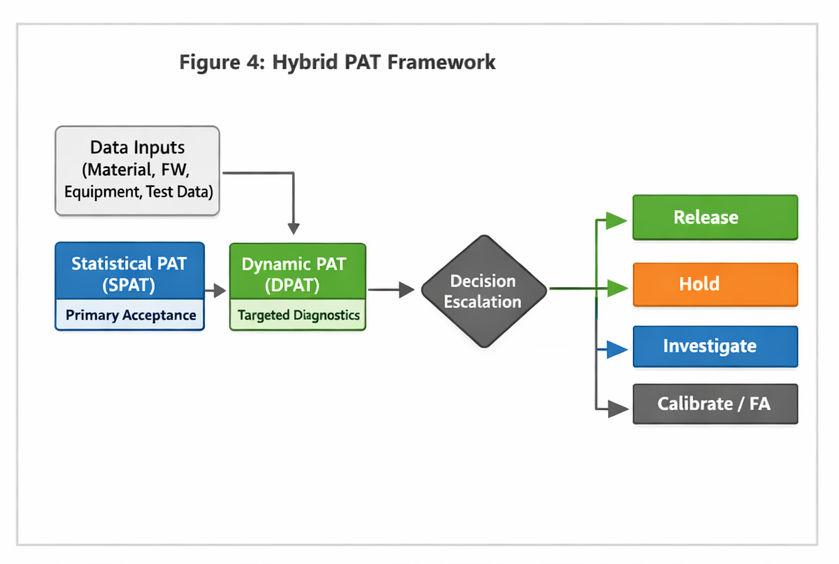
\includegraphics[width=0.92\linewidth]{figures/figure4_hybrid_pat_framework.png}
		\caption{Hybrid framework: SPAT gate + DPAT targeted diagnostics.}
		\label{fig:hybrid}
	\end{figure}
	
	% ---------------------------
	\section{Case Study: Representative MCP Backend Scenario (Illustrative)}
	
	\subsection{Background}
	This scenario represents a typical memory MCP backend manufacturing line where multiple variability sources
	co-exist (BOM mix, FW versions, tester diversity, and contactor wear).
	
	\subsection{Observed issue}
	DPAT flagged abnormal drift in a key parametric metric (Param\_X) and triggered multiple lot holds.
	
	\subsection{Investigation findings}
	Key contributors:
	\begin{itemize}[leftmargin=1.2em]
		\item Firmware revision update changed calibration/training behavior.
		\item Socket/contactor wear introduced gradual measurement bias.
		\item Handler thermal drift amplified non-linear behavior.
	\end{itemize}
	
	\subsection{Root cause}
	The DPAT rolling baseline treated the latest population as “equivalent” although the
	underlying system state changed. This destabilized DPAT thresholds and increased false reject probability.
	
	\subsection{SPAT outcome}
	SPAT baseline remained stable and correctly categorized the effect as a controlled shift, prompting
	targeted tool qualification actions instead of broad product holds.
	
	% ---------------------------
	\section{Simulation Study: Rolling Baseline Fragility in DPAT}
	
	\subsection{Objective}
	To quantify DPAT vs SPAT performance under stacked variability, using a simulated backend system with:
	\begin{itemize}[leftmargin=1.2em]
		\item material source mix (A/B),
		\item firmware version mix (v1/v2),
		\item multiple testers (T1/T2/T3),
		\item socket drift over time,
		\item GR\&R measurement noise.
	\end{itemize}
	
	\subsection{Method}
	We define a synthetic parametric metric $X$ with a base distribution plus additive shifts:
	\[
	X = X_{base} + \Delta_{mat} + \Delta_{fw} + \Delta_{tester} + \Delta_{wear}(t) + \epsilon_{GRR}
	\]
	where $\epsilon_{GRR}$ represents measurement system noise.
	
	\subsection{Evaluation metrics}
	\begin{itemize}[leftmargin=1.2em]
		\item False Reject Rate (FRR)
		\item False Accept Rate (FAR)
		\item Detection lead time under real drift
		\item Threshold stability index (baseline variance)
	\end{itemize}
	
	\subsection{Expected outcome}
	DPAT shows faster detection under stable conditions but degrades significantly when untracked variability
	and baseline drift exist. SPAT remains stable under high-mix conditions.
	
		% ---------------------------
	
	\section{Simulation Study: Multi-Factor Variability Impact on PAT for Read Current}
	
	\subsection{Motivation}
	A common misconception in backend test is that a single parametric metric (e.g., Read Current) reflects only the device behavior.
	In practical backend manufacturing, \textbf{Read Current is a multi-factor system output} influenced by product configuration,
	firmware behavior, test condition variation, and measurement chain effects. As a result, Part Average Testing (PAT) thresholds
	can become unstable, especially when computed using dynamic rolling populations (DPAT).
	
	This simulation study models how stacked variability sources can cause:
	\begin{itemize}[leftmargin=1.2em]
		\item gradual noise accumulation and baseline drift,
		\item periods of apparent stability,
		\item sudden mean shifts caused by discrete changes (e.g., firmware mode mix changes or contact degradation step changes),
		\item increased false rejects/false accepts in DPAT compared to SPAT.
	\end{itemize}
	
	\subsection{Parameter of interest: Read Current}
	Let the key monitored metric be Read Current, denoted as $I_{\text{read}}$.
	Although measured as a single scalar value at test, $I_{\text{read}}$ is affected by:
	\begin{enumerate}[leftmargin=1.2em]
		\item \textbf{Material influence:} material stack and component mix affecting effective resistance, leakage, and timing margin behavior.
		\item \textbf{Firmware speed mode:} high-speed mode requires higher switching activity and performance margin, leading to increased current consumption.
		\item \textbf{Tester/thermal condition:} higher testing temperature increases leakage and can raise current consumption.
		\item \textbf{Measurement chain effects:} degraded contacts, corrosion, or maintenance-related tester leakage introduce additional bias and noise.
	\end{enumerate}
	
	\subsection{Model formulation}
	We model $I_{\text{read}}$ as:
	\[
	I_{\text{read}}(t) = I_0 + \Delta_{\text{mat}} + \Delta_{\text{fw}} + \Delta_T(T) + \Delta_{\text{hw}}(t) + \epsilon(t)
	\]
	
	Where:
	\begin{itemize}[leftmargin=1.2em]
		\item $I_0$: nominal baseline read current
		\item $\Delta_{\text{mat}}$: material-dependent shift (supplier/lot mix)
		\item $\Delta_{\text{fw}}$: firmware mode-dependent shift (fast vs slow operation)
		\item $\Delta_T(T)$: temperature effect term (thermal leakage + dynamic current impact)
		\item $\Delta_{\text{hw}}(t)$: tester HW and contact condition term (slow drift + potential step shifts)
		\item $\epsilon(t)$: measurement noise (GR\&R + local random error)
	\end{itemize}
	
	\subsection{Key assumptions}
	\begin{itemize}[leftmargin=1.2em]
		\item Firmware speed modes are discretized into:
		\begin{itemize}[leftmargin=1.2em]
			\item \textbf{Fast mode} (higher performance): higher $I_{\text{read}}$
			\item \textbf{Slow mode} (lower performance): lower $I_{\text{read}}$
		\end{itemize}
		\item Temperature variation is modeled as a continuous variable, with monotonic impact on current.
		\item Tester hardware condition is modeled as a combination of:
		\begin{itemize}[leftmargin=1.2em]
			\item gradual drift (contact wear / increasing leakage),
			\item occasional sudden step changes (maintenance events, contact failure, or cleaning-driven erosion).
		\end{itemize}
	\end{itemize}
	
	\subsection{Relevance to SPAT vs DPAT}
	In DPAT, thresholds are computed from recent data windows.
	When $I_{\text{read}}$ contains both gradual drift and discrete shifts, dynamic rolling thresholds tend to:
	\begin{itemize}[leftmargin=1.2em]
		\item \textbf{track noise instead of signal} (limit instability),
		\item \textbf{amplify false rejects} during drift,
		\item \textbf{mask escapes} if the rolling window baseline itself degrades.
	\end{itemize}
	
	In SPAT, thresholds derived from long-window historical populations remain stable and robust to short-term variability,
	making SPAT more suitable as the primary acceptance gate in high-mix backend assembly and test.
	
	
	
	% ---------------------------
	\section{Interactive Simulation Extension (Portfolio)}
	
	To enable engineering teams and decision-makers to explore sensitivity interactively, an optional
	interactive simulation environment can be provided via portfolio web application, allowing users to:
	\begin{itemize}[leftmargin=1.2em]
		\item adjust variability sliders (FW, materials, tester mix, GR\&R, wear drift),
		\item observe distribution changes and dynamic threshold movement,
		\item compare SPAT vs DPAT screening behavior.
	\end{itemize}
	
	\textbf{Note:} The interactive simulator uses synthetic data and does not represent any proprietary process limits.
	
	% ---------------------------
	\section{Conclusion}
	Backend assembly and test systems naturally introduce stacked variability and incomplete traceability.
	In such environments, DPAT’s rolling baselines can become unstable and increase false screening decisions.
	SPAT provides a more robust primary screening mechanism. DPAT becomes most effective when backend stability
	and traceability maturity are high. A hybrid approach offers the best practical balance: SPAT gate plus DPAT diagnostics.
	
	% ---------------------------
	\section*{Appendix: Figure List}
	\begin{itemize}[leftmargin=1.2em]
		\item Figure 1: Variance Stack in Backend Assembly \& Test
		\item Figure 2: DPAT Dependency Model
		\item Figure 3: SPAT vs DPAT Comparison Table
		\item Figure 4: Hybrid PAT Framework
	\end{itemize}
	
\end{document}
